\chapter{Seeing What You're Told:\\ Sentence-Guided Activity Recognition In Video}

\section{Introduction}
\label{sec:introduction}
\vspace*{-2ex}
The ability to describe the observed world in natural language is a
quintessential component of human intelligence.
%
A particular feature of this ability is the use of rich sentences, involving
the composition of multiple nouns, adjectives, verbs, adverbs, and
prepositions, to describe not just static objects and scenes, but also events
that unfold over time.
%
Furthermore, this ability appears to be learned by virtually all children.
%
The deep semantic information learned is multi-purpose: it supports
comprehension, generation, and inference.
%
In this work, we investigate the intuition, and the precise means and
mechanisms that will enable us to support such ability in the domain of
activity recognition in multi-activity videos.

Suppose we wanted to recognize an occurrence of an event described by the
sentence \emph{The ball bounced}, in a video.
%
Nominally, we would need to detect the \emph{ball} and its position in the
field of view in each frame and determine that the sequence of such detections
satisfied the requirements of \emph{bounce}.
%
The sequence of such object detections and their corresponding positions over
time constitutes a \defoccur{track} for that object.
%
In this view, the semantics of an intransitive verb like \emph{bounce} would be
formulated as a unary predicate over object tracks.
%
Recognizing occurrences of events described by sentences containing transitive
verbs, like \emph{The person approached the ball}, would require detecting and
tracking two objects, the \emph{person} and the \emph{ball} constrained by a
binary predicate.

In an ideal world, event recognition would proceed in a purely feed-forward
fashion: robust and unambiguous object detection and tracking followed by
application of the semantic predicates on the recovered tracks.
%
However, the current state-of-the-art in computer vision is far from this
ideal.
%
Object detection alone is highly unreliable.
%
The best current average-precision scores on PASCAL VOC hover around 40\%-50\%
\citep{Everingham10}.
%
As a result, object detectors suffer from both false positives and false
negatives.
%
One way around this is to use detection-based tracking \citep{Wolf1989}, where
one biases the detector to overgenerate, alleviating the problem of false
negatives, and uses a different mechanism to select among the overgenerated
detections to alleviate the problem of false positives.
%
One such mechanism selects detections that are temporally coherent, \ie\ the
track motion being consistent with optical flow.
%
\cite{Barbu2012b} proposed an alternate mechanism that selected detections for
a track that satisfied a unary predicate such as one would construct for an
intransitive verb like \emph{bounce}.
%
We significantly extend that approach, selecting detections for multiple tracks
that collectively satisfy a complex multi-argument predicate representing the
semantics of an entire sentence.
%
That predicate is constructed as a conjunction of predicates representing the
semantics of the individual words in that sentence.
%
For example, given the sentence \emph{The person to the left of the chair
  approached the trash can}, we construct a logical form.
%
\begin{equation*}
% \vspace*{-1ex}
  \textsc{person}(P)\wedge
  \textsc{toTheLeftOf}(P,Q)\wedge
  \textsc{chair}(Q)\wedge
  \textsc{approach}(P,R)\wedge
  \textsc{trashCan}(R)
\end{equation*}
%
Our tracker is able to simultaneously construct three tracks~$P$, $Q$, and~$R$,
selecting out detections for each, in an optimal fashion that simultaneously
optimizes a joint measure of detection score and temporal coherence while also
satisfying the above conjunction of predicates.
%
We obtain the aforementioned detections by employing a state-of-the-art object
detector \citep{Felzenszwalb2010b}, where we train a model for each object
(\eg\ \emph{person}, \emph{chair}, \etc), which when applied to an image,
produces axis-aligned bounding boxes with associated scores indicating strength
of detection.

We represent the semantics of lexical items like \emph{person}, \emph{to the
  left of}, \emph{chair}, \emph{approach}, and \emph{trash can} with predicates
over tracks like $\textsc{person}(P)$, $\textsc{toTheLeftOf}(P,Q)$,
$\textsc{chair}(Q)$, $\textsc{approach}(P,R)$, and $\textsc{trashCan}(R)$.
%
% needs work: temporal derivatives
%
These predicates are in turn represented as regular expressions (\ie\ finite
state recognizers or FSMs) over features extracted from the sequence of
detection positions, shapes, and sizes as well as their temporal derivatives.
%
For example, the predicate $\textsc{toTheLeftOf}(P,Q)$ might be a single state
FSM where, on a frame-by-frame basis, the centers of the detections for~$P$ are
constrained to have a lower $x$-coordinate than the centers of the detections
for~$Q$.
%
The actual formulation of the predicates (Table~\ref{tab:predicates}) is far
more complex to deal with noise and variance in real-world video.
%
What is central is that the semantics of \emph{all} parts of speech, namely
nouns, adjectives, verbs, adverbs, and prepositions (both those that describe
spatial-relations and those that describe motion), is uniformly represented by
the same mechanism: predicates over tracks formulated as finite state
recognizers over features extracted from the detections in those tracks.

We refer to this capacity as the \defoccur{Sentence Tracker}, which is a
function $\mathcal{S}:(D,\Phi)\mapsto(\tau,Z)$, that takes as input an
overgenerated set~$D$ of detections along with a complex sentential
predicate~$\Phi$ and produces a score~$\tau$ together with a set~$Z$ of tracks
that satisfy~$\Phi$ while optimizing a linear combination of detection scores
and temporal coherence.
%
This can be used for three distinct purposes:
%
\vspace*{-3ex}
\begin{compactdesc}
  %
\item[focus of attention] One can apply the sentence tracker to the same
  video~$D$, that depicts multiple simultaneous events taking place in the
  field of view with different participants, with two different
  sentences~$\Phi_1$ and~$\Phi_2$.
  %
  In other words, one can compute $(\tau_1,Z_1)=\mathcal{S}(D,\Phi_1)$ and
  $(\tau_2,Z_2)=\mathcal{S}(D,\Phi_2)$ to yield two different sets of
  tracks~$Z_1$ and~$Z_2$ corresponding to the different sets of participants in
  the different events described by~$\Phi_1$ and~$\Phi_2$.
  %
  We demonstrate this in section~\ref{subsec:foa}.
  %
\item[generation] One can take a video~$D$ as input and systematically search
  the space of all possible~$\Phi$ that correspond to sentences that can be
  generated by a context-free grammar and find that sentence that corresponds
  to the~$\Phi^{*}$ for which $(\tau^{*},Z^{*})=\mathcal{S}(D,\Phi^{*})$ yields
  the maximal~$\tau^{*}$.
  %
  This can be used to generate a sentence that describes an input video~$D$.
  %
  We demonstrate this in section~\ref{subsec:generation}.
  %
\item[retrieval] One can take a collection~$\mathcal{D}=\{D_1,\ldots,D_n\}$ of
  videos (or a single long video temporally segmented into short clips) along
  with a sentential query~$\Phi$, compute $(\tau_i,Z_i)=\mathcal{S}(D_i,\Phi)$
  for each~$D_i$, and find the clip~$D_i$ with maximal score~$\tau_i$.
  %
  This can be used to perform sentence-based video search.
  %
  We demonstrate this in section~\ref{subsec:retrieval}.
  %
\end{compactdesc}
\vspace*{-1ex}
%
However, we first present the two central algorithmic contributions of this
work.
%
In section~\ref{sec:tracker} we present the details of the sentence tracker,
the mechanism for efficiently constraining several parallel detection-based
trackers, one for each participant, with a conjunction of finite state
recognizers.
%
In section~\ref{sec:semantics} we present lexical semantics for a small
vocabulary of~17 lexical items (5~nouns, 2~adjectives, 4~verbs, 2~adverbs,
2~spatial-relation prepositions, and 2~motion prepositions) all formulated as
finite state recognizers over features extracted from detections produced by an
object detector, together with compositional semantics that maps a sentence to
a semantic formula~$\Phi$ constructed from these finite state recognizers where
the object tracks are assigned to arguments of these recognizers.

\vspace*{-2ex}
\section{The Sentence Tracker}
\label{sec:tracker}
\vspace*{-2ex}

\citet{Barbu2012b} address the issue of selecting detections for a track that
simultaneously satisfies a temporal-coherence measure and a single predicate
corresponding to an intransitive verb such as \emph{bounce}.
%
Doing so constitutes the integration of top-down high-level information, in the
form of an event model, with bottom-up low-level information in the form of
object detectors.
%
We provide a short review of the relevant material in that work to introduce
notation and provide the basis for our exposition of the sentence tracker.

\begin{wrapfigure}{r}{0.44\textwidth}
  \vspace*{-3.5ex}
  \begin{center}
    \begin{minipage}[b]{0.44\textwidth}
      \begin{equation}
        \max_{j^1,\ldots,j^T}
        \sum_{t=1}^Tf(b^t_{j^t})+\sum_{t=2}^Tg(b^{t-1}_{j^{t-1}},b^t_{j^t})
        \label{eq:tracker}
      \end{equation}
    \end{minipage}
  \end{center}
  \vspace*{-4ex}
\end{wrapfigure}
%
The first component is a detection-based tracker.
%
For a given video with~$T$ frames, let~$j$ be the index of a detection
and~$b^t_j$ be a particular detection in frame~$t$ with score $f(b^t_j)$.
%
A sequence $\langle j^1,\ldots,j^T\rangle$ of detection indices, one for each
frame~$t$, denotes a track comprising detections $b^t_{j^t}$.
%
We seek a track that maximizes a linear combination of aggregate detection
score, summing $f(b^t_j)$ over all frames, and a measure of temporal coherence,
as formulated in Eq.~\ref{eq:tracker}.
%
The temporal coherence measure aggregates a local measure~$g$ computed between
pairs of adjacent frames, taken to be the negative Euclidean distance between
the center of $b^t_{j^t}$ and the forward-projected center of
$b^{t-1}_{j^{t-1}}$ computed with optical flow.
%
Eq.~\ref{eq:tracker} can be computed in polynomial time using
dynamic-programming with the \citet{Viterbi1971} algorithm.
%
It does so by formulating a lattice, whose rows are indexed by~$j$ and whose
columns are indexed by~$t$, where the node at row~$j$ and column~$t$ is the
detection $b^t_j$.
%
Finding a track thus reduces to finding a path through this lattice.

\begin{wrapfigure}{r}{0.45\textwidth}
  \vspace*{-6.5ex}
  \begin{center}
    \begin{minipage}[b]{0.45\textwidth}
      \begin{equation}
        \max_{k^1,\ldots,k^T}
        \sum_{t=1}^Th(k^t,b^t_{\hat{\jmath}^t})+\sum_{t=2}^Ta(k^{t-1},k^t)
        \label{eq:map}
      \end{equation}
    \end{minipage}
  \end{center}
  \vspace*{-3ex}
\end{wrapfigure}
%
The second component recognizes events with hidden Markov models (HMMs), by
finding a maximum \emph{a posteriori} probability (MAP) estimate of an event
model given a track.
%
This is computed as shown in Eq.~\ref{eq:map}, where~$k^t$ denotes the
state for frame~$t$, $h(k,b)$ denotes the log probability of generating a
detection~$b$ conditioned on being in state~$k$, $a(k',k)$ denotes the log
probability of transitioning from state~$k'$ to~$k$, and $\hat{\jmath}^t$
denotes the index of the detection produced by the tracker in frame~$t$.
%
This can also be computed in polynomial time using the Viterbi algorithm.
%
Doing so induces a lattice, whose rows are indexed by~$k$ and whose columns are
indexed by~$t$.

The two components, detection-based tracking and event recognition, can be
combined.
One can combine the cost functions from Eq.~\ref{eq:tracker} and
Eq.~\ref{eq:map} to yield a unified cost function
%
\begin{equation*}
  \max_{\substack{j^1,\ldots,j^T\\k^1,\ldots,k^T}}
  \displaystyle\sum_{t=1}^T f(b^t_{j^t})
  +\displaystyle\sum_{t=2}^T g(b^{t-1}_{j^{t-1}},b^t_{j^t})
  +\displaystyle\sum_{t=1}^Th(k^t,b^t_{j^t})
  +\displaystyle\sum_{t=2}^Ta(k^{t-1},k^t)
\end{equation*}
%
that computes the joint MAP estimate of the best possible track and the best
possible state sequence.
%
This is done by replacing the $\hat{\jmath}^t$ in Eq.~\ref{eq:map} with~$j^t$,
allowing the joint maximization over detection and state sequences.
%
This too can be computed in polynomial time with the Viterbi algorithm, finding
the optimal path through a cross-product lattice where each node represents a
detection paired with an event-model state.
%
This formulation combines a single tracker lattice with a single event model,
constraining the detection-based tracker to find a track that is not only
temporally coherent but also satisfies the event model.
%
This can be used to select that \emph{ball} track from a video that contains
multiple balls that exhibits the motion characteristics of an intransitive verb
such as \emph{bounce}.

\begin{wrapfigure}{r}{0.47\textwidth}
  \vspace*{-4.5ex}
  \begin{center}
    \begin{tabular}{@{}c@{\hspace*{5pt}}c@{\hspace*{5pt}}c@{}}
      track $1$&&track $L$\\
      \scalebox{0.17}{\input{figures/viterbi-tracker-1}}&
      \raisebox{15pt}{{\Large $\times\cdots\times$}}&
      \scalebox{0.17}{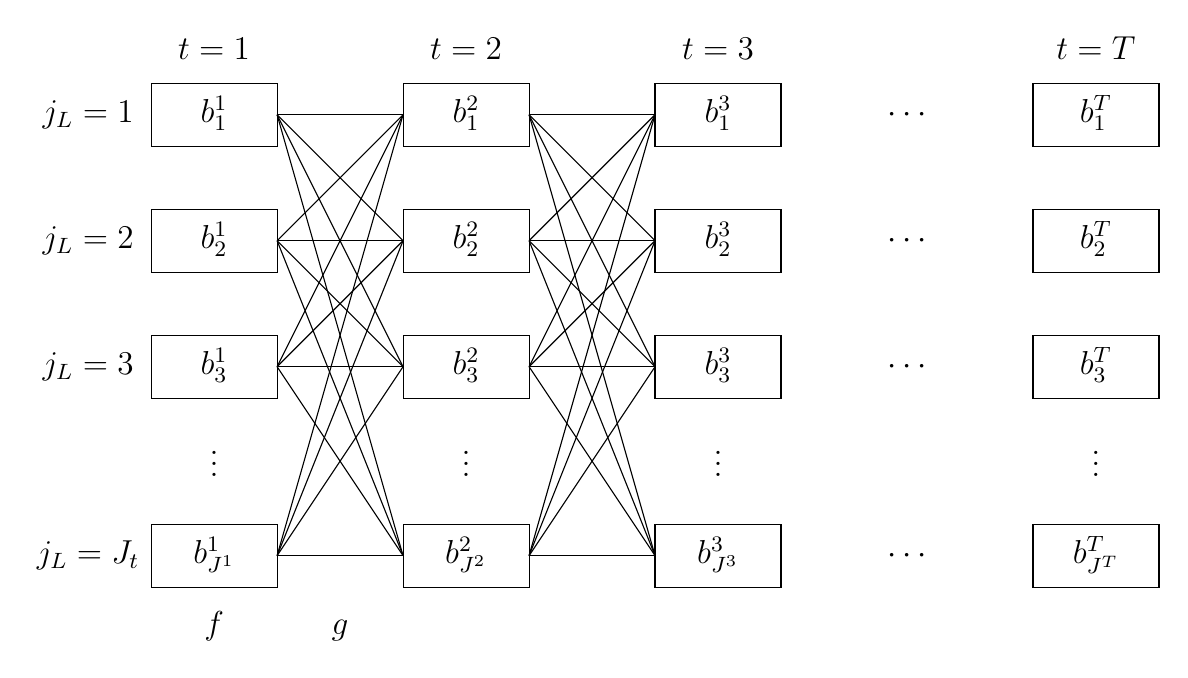
\begin{tikzpicture}[y=-1cm]

% objects at depth 50:
\draw[black] (3.8,4.2) -- (5.4,4.2);
\draw[black] (3.8,2.6) -- (5.4,2.6);
\draw[black] (3.8,5.8) -- (5.4,5.8);
\draw[black] (3.8,8.2) -- (5.4,8.2);
\draw[black] (3.8,2.6) -- (5.4,4.2);
\draw[black] (3.8,2.6) -- (5.4,5.8);
\draw[black] (3.8,2.6) -- (5.4,8.2);
\draw[black] (3.8,4.2) -- (5.4,2.6);
\draw[black] (3.8,4.2) -- (5.4,5.8);
\draw[black] (3.8,4.2) -- (5.4,8.2);
\draw[black] (3.8,5.8) -- (5.4,2.6);
\draw[black] (3.8,5.8) -- (5.4,4.2);
\draw[black] (3.8,5.8) -- (5.4,8.2);
\draw[black] (3.8,8.2) -- (5.4,2.6);
\draw[black] (3.8,8.2) -- (5.4,4.2);
\draw[black] (3.8,8.2) -- (5.4,5.8);
\draw[black] (7,4.2) -- (8.6,4.2);
\draw[black] (7,2.6) -- (8.6,2.6);
\draw[black] (7,5.8) -- (8.6,5.8);
\draw[black] (7,8.2) -- (8.6,8.2);
\draw[black] (7,2.6) -- (8.6,4.2);
\draw[black] (7,2.6) -- (8.6,5.8);
\draw[black] (7,2.6) -- (8.6,8.2);
\draw[black] (7,4.2) -- (8.6,2.6);
\draw[black] (7,4.2) -- (8.6,5.8);
\draw[black] (7,4.2) -- (8.6,8.2);
\draw[black] (7,5.8) -- (8.6,2.6);
\draw[black] (7,5.8) -- (8.6,4.2);
\draw[black] (7,5.8) -- (8.6,8.2);
\draw[black] (7,8.2) -- (8.6,2.6);
\draw[black] (7,8.2) -- (8.6,4.2);
\draw[black] (7,8.2) -- (8.6,5.8);
\draw[black] (2.2,2.2) rectangle (3.8,3);
\draw[black] (2.2,3.8) rectangle (3.8,4.6);
\draw[black] (2.2,5.4) rectangle (3.8,6.2);
\draw[black] (2.2,7.8) rectangle (3.8,8.6);
\path (3,7.2) node[text=black,anchor=base] {\large{}$\vdots$};
\draw[black] (8.6,2.2) rectangle (10.2,3);
\draw[black] (8.6,3.8) rectangle (10.2,4.6);
\draw[black] (8.6,5.4) rectangle (10.2,6.2);
\draw[black] (8.6,7.8) rectangle (10.2,8.6);
\path (9.4,7.2) node[text=black,anchor=base] {\large{}$\vdots$};
\draw[black] (13.4,2.2) rectangle (15,3);
\draw[black] (13.4,3.8) rectangle (15,4.6);
\draw[black] (13.4,5.4) rectangle (15,6.2);
\draw[black] (13.4,7.8) rectangle (15,8.6);
\path (14.2,7.2) node[text=black,anchor=base] {\large{}$\vdots$};
\draw[black] (5.4,2.2) rectangle (7,3);
\draw[black] (5.4,3.8) rectangle (7,4.6);
\draw[black] (5.4,5.4) rectangle (7,6.2);
\draw[black] (5.4,7.8) rectangle (7,8.6);
\path (6.2,7.2) node[text=black,anchor=base] {\large{}$\vdots$};
\path (3,9.2) node[text=black,anchor=base] {\large{}$f$};
\path (4.6,9.2) node[text=black,anchor=base] {\large{}$g$};
\path (3,1.9) node[text=black,anchor=base] {\large{}$t=1$};
\path (6.2,1.9) node[text=black,anchor=base] {\large{}$t=2$};
\path (9.4,1.9) node[text=black,anchor=base] {\large{}$t=3$};
\path (14.2,1.9) node[text=black,anchor=base] {\large{}$t=T$};
\path (1.4,2.7) node[text=black,anchor=base] {\large{}$j_L=1$};
\path (1.4,5.9) node[text=black,anchor=base] {\large{}$j_L=3$};
\path (1.4,4.3) node[text=black,anchor=base] {\large{}$j_L=2$};
\path (1.4,8.3) node[text=black,anchor=base] {\large{}$j_L=J_t$};
\path (3,2.7) node[text=black,anchor=base] {\large{}$b^1_1$};
\path (3,4.3) node[text=black,anchor=base] {\large{}$b^1_2$};
\path (3,5.9) node[text=black,anchor=base] {\large{}$b^1_3$};
\path (6.2,2.7) node[text=black,anchor=base] {\large{}$b^2_1$};
\path (6.2,4.3) node[text=black,anchor=base] {\large{}$b^2_2$};
\path (6.2,5.9) node[text=black,anchor=base] {\large{}$b^2_3$};
\path (9.4,2.7) node[text=black,anchor=base] {\large{}$b^3_1$};
\path (9.4,4.3) node[text=black,anchor=base] {\large{}$b^3_2$};
\path (9.4,5.9) node[text=black,anchor=base] {\large{}$b^3_3$};
\path (14.2,2.7) node[text=black,anchor=base] {\large{}$b^T_1$};
\path (14.2,4.3) node[text=black,anchor=base] {\large{}$b^T_2$};
\path (14.2,5.9) node[text=black,anchor=base] {\large{}$b^T_3$};
\path (3,8.3) node[text=black,anchor=base] {\large{}$b^1_{J^1}$};
\path (6.2,8.3) node[text=black,anchor=base] {\large{}$b^2_{J^2}$};
\path (9.4,8.3) node[text=black,anchor=base] {\large{}$b^3_{J^3}$};
\path (14.2,8.3) node[text=black,anchor=base] {\large{}$b^T_{J^T}$};
\path (11.8,2.7) node[text=black,anchor=base] {\large{}$\cdots$};
\path (11.8,4.3) node[text=black,anchor=base] {\large{}$\cdots$};
\path (11.8,5.9) node[text=black,anchor=base] {\large{}$\cdots$};
\path (11.8,8.3) node[text=black,anchor=base] {\large{}$\cdots$};

\end{tikzpicture}%
}\\[-0.5ex]
      &\raisebox{5pt}{{\huge $\times$}}&\\[-0.5ex]
      \scalebox{0.17}{\input{figures/sentence-tracker-1}}&
      \raisebox{15pt}{{\Large $\times\cdots\times$}}&
      \scalebox{0.17}{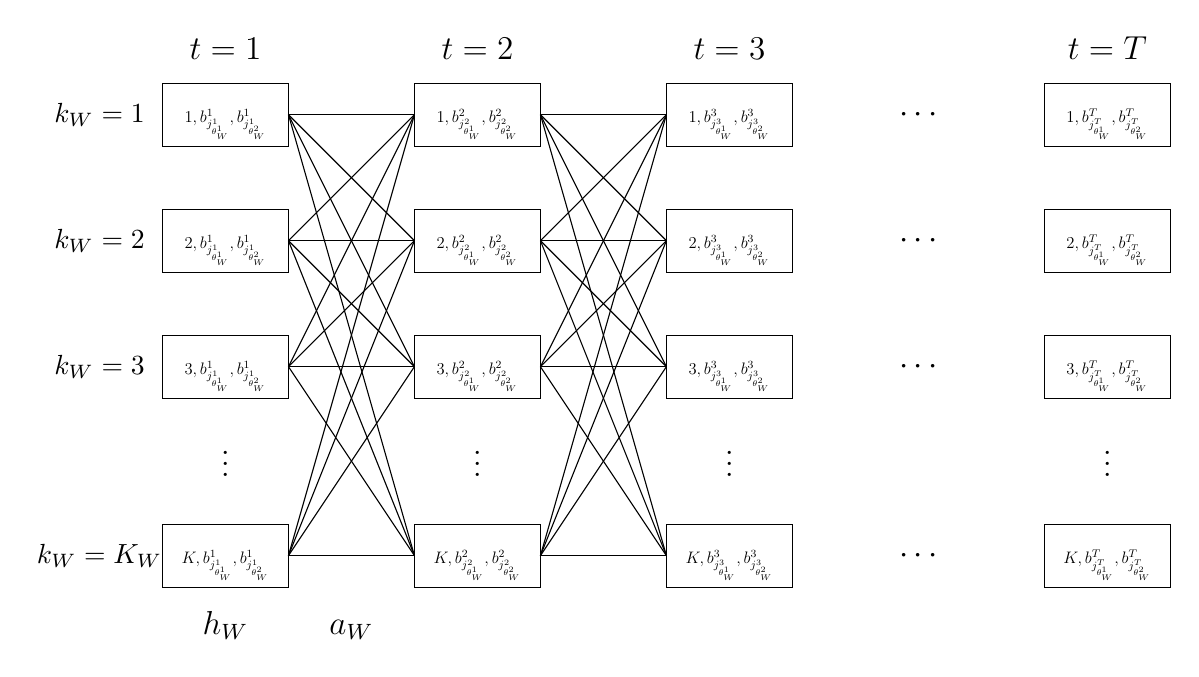
\begin{tikzpicture}[y=-1cm]

% objects at depth 50:
\draw[black] (3.8,4.2) -- (5.4,4.2);
\draw[black] (3.8,2.6) -- (5.4,2.6);
\draw[black] (3.8,5.8) -- (5.4,5.8);
\draw[black] (3.8,8.2) -- (5.4,8.2);
\draw[black] (3.8,2.6) -- (5.4,4.2);
\draw[black] (3.8,2.6) -- (5.4,5.8);
\draw[black] (3.8,2.6) -- (5.4,8.2);
\draw[black] (3.8,4.2) -- (5.4,2.6);
\draw[black] (3.8,4.2) -- (5.4,5.8);
\draw[black] (3.8,4.2) -- (5.4,8.2);
\draw[black] (3.8,5.8) -- (5.4,2.6);
\draw[black] (3.8,5.8) -- (5.4,4.2);
\draw[black] (3.8,5.8) -- (5.4,8.2);
\draw[black] (3.8,8.2) -- (5.4,2.6);
\draw[black] (3.8,8.2) -- (5.4,4.2);
\draw[black] (3.8,8.2) -- (5.4,5.8);
\draw[black] (7,4.2) -- (8.6,4.2);
\draw[black] (7,2.6) -- (8.6,2.6);
\draw[black] (7,5.8) -- (8.6,5.8);
\draw[black] (7,8.2) -- (8.6,8.2);
\draw[black] (7,2.6) -- (8.6,4.2);
\draw[black] (7,2.6) -- (8.6,5.8);
\draw[black] (7,2.6) -- (8.6,8.2);
\draw[black] (7,4.2) -- (8.6,2.6);
\draw[black] (7,4.2) -- (8.6,5.8);
\draw[black] (7,4.2) -- (8.6,8.2);
\draw[black] (7,5.8) -- (8.6,2.6);
\draw[black] (7,5.8) -- (8.6,4.2);
\draw[black] (7,5.8) -- (8.6,8.2);
\draw[black] (7,8.2) -- (8.6,2.6);
\draw[black] (7,8.2) -- (8.6,4.2);
\draw[black] (7,8.2) -- (8.6,5.8);
\draw[black] (5.4,2.2) rectangle (7,3);
\draw[black] (5.4,3.8) rectangle (7,4.6);
\draw[black] (5.4,5.4) rectangle (7,6.2);
\draw[black] (5.4,7.8) rectangle (7,8.6);
\path (6.2,7.2) node[text=black,anchor=base] {\large{}$\vdots$};
\draw[black] (8.6,2.2) rectangle (10.2,3);
\draw[black] (8.6,3.8) rectangle (10.2,4.6);
\draw[black] (8.6,5.4) rectangle (10.2,6.2);
\draw[black] (8.6,7.8) rectangle (10.2,8.6);
\path (9.4,7.2) node[text=black,anchor=base] {\large{}$\vdots$};
\draw[black] (2.2,2.2) rectangle (3.8,3);
\draw[black] (2.2,3.8) rectangle (3.8,4.6);
\draw[black] (2.2,5.4) rectangle (3.8,6.2);
\draw[black] (2.2,7.8) rectangle (3.8,8.6);
\path (3,7.2) node[text=black,anchor=base] {\large{}$\vdots$};
\draw[black] (13.4,2.2) rectangle (15,3);
\draw[black] (13.4,3.8) rectangle (15,4.6);
\draw[black] (13.4,5.4) rectangle (15,6.2);
\draw[black] (13.4,7.8) rectangle (15,8.6);
\path (14.2,7.2) node[text=black,anchor=base] {\large{}$\vdots$};
\path (3,1.9) node[text=black,anchor=base] {\large{}$t=1$};
\path (6.2,1.9) node[text=black,anchor=base] {\large{}$t=2$};
\path (9.4,1.9) node[text=black,anchor=base] {\large{}$t=3$};
\path (14.2,1.9) node[text=black,anchor=base] {\large{}$t=T$};
\path (1.4,2.7) node[text=black,anchor=base] {$k_W=1$};
\path (1.4,4.3) node[text=black,anchor=base] {$k_W=2$};
\path (1.4,8.3) node[text=black,anchor=base] {$k_W=K_W$};
\path (1.4,5.9) node[text=black,anchor=base] {$k_W=3$};
\path (3,9.2) node[text=black,anchor=base] {\large{}$h_W$};
\path (4.6,9.2) node[text=black,anchor=base] {\large{}$a_W$};
\path (11.8,2.7) node[text=black,anchor=base] {\large{}$\cdots$};
\path (11.8,4.3) node[text=black,anchor=base] {\large{}$\cdots$};
\path (11.8,5.9) node[text=black,anchor=base] {\large{}$\cdots$};
\path (11.8,8.3) node[text=black,anchor=base] {\large{}$\cdots$};
\path (3,2.7) node[text=black,anchor=base] {\large{}\scalebox{0.5}{$1,b^1_{j^1_{\theta^1_W}},b^1_{j^1_{\theta^2_W}}$}};
\path (3,4.3) node[text=black,anchor=base] {\large{}\scalebox{0.5}{$2,b^1_{j^1_{\theta^1_W}},b^1_{j^1_{\theta^2_W}}$}};
\path (3,5.9) node[text=black,anchor=base] {\large{}\scalebox{0.5}{$3,b^1_{j^1_{\theta^1_W}},b^1_{j^1_{\theta^2_W}}$}};
\path (3,8.3) node[text=black,anchor=base] {\large{}\scalebox{0.5}{$K,b^1_{j^1_{\theta^1_W}},b^1_{j^1_{\theta^2_W}}$}};
\path (6.2,2.7) node[text=black,anchor=base] {\large{}\scalebox{0.5}{$1,b^2_{j^2_{\theta^1_W}},b^2_{j^2_{\theta^2_W}}$}};
\path (6.2,4.3) node[text=black,anchor=base] {\large{}\scalebox{0.5}{$2,b^2_{j^2_{\theta^1_W}},b^2_{j^2_{\theta^2_W}}$}};
\path (6.2,5.9) node[text=black,anchor=base] {\large{}\scalebox{0.5}{$3,b^2_{j^2_{\theta^1_W}},b^2_{j^2_{\theta^2_W}}$}};
\path (6.2,8.3) node[text=black,anchor=base] {\large{}\scalebox{0.5}{$K,b^2_{j^2_{\theta^1_W}},b^2_{j^2_{\theta^2_W}}$}};
\path (9.4,2.7) node[text=black,anchor=base] {\large{}\scalebox{0.5}{$1,b^3_{j^3_{\theta^1_W}},b^3_{j^3_{\theta^2_W}}$}};
\path (9.4,4.3) node[text=black,anchor=base] {\large{}\scalebox{0.5}{$2,b^3_{j^3_{\theta^1_W}},b^3_{j^3_{\theta^2_W}}$}};
\path (9.4,5.9) node[text=black,anchor=base] {\large{}\scalebox{0.5}{$3,b^3_{j^3_{\theta^1_W}},b^3_{j^3_{\theta^2_W}}$}};
\path (9.4,8.3) node[text=black,anchor=base] {\large{}\scalebox{0.5}{$K,b^3_{j^3_{\theta^1_W}},b^3_{j^3_{\theta^2_W}}$}};
\path (14.2,2.7) node[text=black,anchor=base] {\large{}\scalebox{0.5}{$1,b^T_{j^T_{\theta^1_W}},b^T_{j^T_{\theta^2_W}}$}};
\path (14.2,4.3) node[text=black,anchor=base] {\large{}\scalebox{0.5}{$2,b^T_{j^T_{\theta^1_W}},b^T_{j^T_{\theta^2_W}}$}};
\path (14.2,5.9) node[text=black,anchor=base] {\large{}\scalebox{0.5}{$3,b^T_{j^T_{\theta^1_W}},b^T_{j^T_{\theta^2_W}}$}};
\path (14.2,8.3) node[text=black,anchor=base] {\large{}\scalebox{0.5}{$K,b^T_{j^T_{\theta^1_W}},b^T_{j^T_{\theta^2_W}}$}};

\end{tikzpicture}%
}\\[-0.5ex]
      word $1$&&word $W$
    \end{tabular}
  \end{center}
  \vspace*{-3ex}
  \caption{The cross-product lattice used by the sentence tracker, consisting
    of~$L$ tracking lattices and~$W$ event-model lattices.}
  \label{fig:sentence-tracker}
  \vspace*{-2ex}
\end{wrapfigure}
%
One would expect that encoding the semantics of a complex sentence such as
\emph{The person to the right of the chair quickly carried the red object
  towards the trash can}, which involves nouns, adjectives, verbs, adverbs, and
spatial-relation and motion prepositions, would provide substantially more
mutual constraint on the \emph{collection} of tracks for the participants than a
single intransitive verb would constrain a single track.
%
We thus extend the approach described above by incorporating a complex
multi-argument predicate that represents the semantics of an entire sentence
instead of one that only represents the semantics of a single intransitive verb.
%
This involves formulating the semantics of other parts of speech, in addition
to intransitive verbs, also as HMMs.
%
We then construct a large cross-product lattice, illustrated in
Fig.~\ref{fig:sentence-tracker}, to support~$L$ tracks and~$W$ words.
%
Each node in this cross-product lattice represents $L$~detections and the
states for~$W$ words.
%
To support~$L$ tracks, we subindex each detection index~$j$ as $j_l$ for
track~$l$.
%
Similarly, to support~$W$ words, we subindex each state index~$k$ as~$k_w$ for
word~$w$ and the HMM parameters~$h$ and~$a$ for word~$w$ as~$h_w$ and~$a_w$.
%
The argument-to-track mappings~$\theta^1_w$ and~$\theta^2_w$ specify the tracks
that fill arguments~1 and~2 (where necessary) of word~$w$ respectively.
%
We then seek a path through this cross-product lattice that optimizes
%
\vspace*{-2ex}
\begin{equation*}
  \max_{\substack{j^1_1,\ldots,j^T_1\\j^1_L,\ldots,j^T_L\\
      k^1_1,\ldots,k^T_1\\k^1_W,\ldots,k^T_W}}
  \sum_{l=1}^L
  \sum_{t=1}^Tf(b^t_{j^t_l})+
  \sum_{t=2}^Tg(b^{t-1}_{j^{t-1}_l},b^t_{j^t_l})+
  \sum_{w=1}^W
  \sum_{t=1}^Th_w(k^t_w,b^t_{j^t_{\theta^1_w}},b^t_{j^t_{\theta^2_w}})+
  \sum_{t=2}^Ta_w(k^{t-1}_w,k^t_w)
\end{equation*}
%
This can also be computed in polynomial time using the Viterbi algorithm.
%
This describes a method by which the function
$\mathcal{S}(D,\Phi)\mapsto(\tau,Z)$, discussed earlier, can be computed, where
$D$~is the collection of detections~$b^t_j$ and~$Z$ is the collection of
tracks~$j^t_l$.

\vspace*{-2ex}
\section{Natural-Language Semantics}
\label{sec:semantics}
\vspace*{-2ex}

The sentence tracker uniformly represents the semantics of words in all parts
of speech, namely nouns, adjectives, verbs, adverbs, and prepositions (both
those that describe spatial relations and those that describe motion), as HMMs.
%
Finite state recognizers (FSMs) are a special case of HMMs where the transition
matrices~$a$ and the output models~$h$ are 0/1.
%
Here, we formulate the semantics of a small fragment of English consisting
of~17 lexical items (5~nouns, 2~adjectives, 4~verbs, 2~adverbs,
2~spatial-relation prepositions, and 2~motion prepositions), by hand, as FSMs.
%
We do so to focus on what once can do with this approach, namely take sentences
as input and focus the attention of a tracker, take video as input and produce
sentential descriptions as output, and perform content-based video retrieval
given a sentential input query, as discussed in Section~\ref{sec:experiments}.
%
It is particularly enlightening that the FSMs we use are perspicuous and
clearly encode pretheoretic human intuitions about the semantics of these words.
%
But nothing turns on the use of hand-coded FSMs.
%
Our framework, as described above, supports HMMs.
%
A companion submission describes a method by which one can automatically learn
such HMMs for the lexicon, grammar, and corpus discussed in this paper.

\begin{table}[t]
  \centering\ra{1.1}
  \begin{tabular}{@{}cc@{}}
    \begin{tabular}{@{}c@{}}
      \scalebox{0.65}{\begin{tabular}{@{}r@{$\;\rightarrow\;$}l@{}}
        S & NP VP\\
        NP & D [A] N [PP]\\
        D & \emph{an} \textbar\ \emph{the}\\
        A & \emph{blue} \textbar\ \emph{red}\\
        N & \emph{person} \textbar\ \emph{backpack} \textbar\ \emph{trash can} \textbar\ \emph{chair} \textbar\ \emph{object}\\
        PP & P NP\\
        P & \emph{to the left of} \textbar\ \emph{to the right of}\\
        VP & V NP [ADV] [PPM]\\
        V & \emph{picked up} \textbar\ \emph{put down} \textbar\ \emph{carried} \textbar\ \emph{approached}\\
        ADV & \emph{quickly} \textbar\ \emph{slowly}\\
        PPM & PM NP\\
        PM & \emph{towards} \textbar\ \emph{away from}
      \end{tabular}}\\
      (a)\\
      \scalebox{0.65}{\begin{tabular}{@{}r@{$\;=\;$}l@{}}
          \emph{to the left of} & (agent patient) (referent)\\
          \emph{to the right of} & (agent patient) (referent)\\
          \emph{picked up} & (agent) (patient)\\
          \emph{put down} & (agent) (patient)\\
          \emph{carried} & (agent) (patient)\\
          \emph{approached} & (agent) (goal)\\
          \emph{towards} & (agent patient) (goal)\\
          \emph{away from} & (agent patient) (source)\\
          other & (agent patient referent goal source)\\
      \end{tabular}}\\
      (b)
    \end{tabular}&
  \begin{tabular}{@{}c@{}}
    \scalebox{0.7}{\begin{tabular}{@{}r@{}l@{.\hspace{1ex}}l@{}}
        1&a&\emph{The backpack approached the trash can.}\\
        &b&\emph{The chair approached the trash can.}\\
        2&a&\emph{The red object approached the chair.}\\
        &b&\emph{The blue object approached the chair.}\\
        3&a&\emph{The person to the left of the trash can put down an object.}\\
        &b&\emph{The person to the right of the trash can put down an object.}\\
        4&a&\emph{The person put down the trash can.}\\
        &b&\emph{The person put down the backpack.}\\
        5&a&\emph{The person carried the red object.}\\
        &b&\emph{The person carried the blue object.}\\
        6&a&\emph{The person picked up an object to the left of the trash can.}\\
        &b&\emph{The person picked up an object to the right of the trash can.}\\
        7&a&\emph{The person picked up an object.}\\
        &b&\emph{The person put down an object.}\\
        8&a&\emph{The person picked up an object quickly.}\\
        &b&\emph{The person picked up an object slowly.}\\
        9&a&\emph{The person carried an object towards the trash can.}\\
        &b&\emph{The person carried an object away from the trash can.}\\
        1&0&\emph{The backpack approached the chair.}\\
        1&1&\emph{The red object approached the trash can.}\\
        1&2&\emph{The person put down the chair.}
    \end{tabular}}\\
    (c)
    \end{tabular}
  \end{tabular}
  \vspace*{-2ex}
  \caption{(a) The grammar for our lexicon of 19 lexical entries (2
    determiners, 2 adjectives, 5 nouns, 2 spatial relations, 4 verbs, 2
    adverbs, and 2 motion prepositions).
    %
    Note that the grammar allows for infinite recursion in the noun phrase.
    %
    (b) The theta grid, specifying the number of arguments and
    roles such arguments refer to, for our lexicon.
    %
    (c) A selection of sentences drawn from the grammar based on which we
    collected (multiple instances of) videos for our experimental corpus..  }
  \label{tab:language}
  \vspace*{-3ex}
\end{table}

Nouns (\eg\ \emph{person}) may be represented by constructing static FSMs over
discrete features, such as detector class.
%
Adjectives (\eg\ \emph{red}, \emph{tall}, and \emph{big}) may be represented as
static FSMs that describe select properties of the detections for a single
participant, such as color, shape, or size, independent of other features of
the overall event.
%
Intransitive verbs (\eg\ \emph{bounce}) may be represented as FSMs that
describe the changing motion characteristics of a single participant, such as
\emph{moving downward} followed by \emph{moving upward}.
%
Transitive verbs (\eg\ \emph{approach}) may be represented as FSMs that
describe the changing relative motion characteristics of two participants, such
as \emph{moving closer}.
%
Adverbs (\eg\ \emph{slowly} and \emph{quickly}) may be represented by FSMs that
describe the velocity of a single participant, independent of the direction of
motion.
%
Spatial-relation prepositions (\eg\ \emph{to the left of}) may be represented
as static FSMs that describe the relative position of two participants.
%
Motion prepositions (\eg\ \emph{towards} and \emph{away from}) may be
represented as FSMs that describe the changing relative position of two
participants.
%
As is often the case, even simple static properties, such as detector class,
object color, shape, and size, spatial relations, and direction of motion,
might hold only for a portion of an event.
%
We handle such temporal uncertainty by incorporating garbage states into the
FSMs that always accept and do not affect the scores computed.
%
This also allows for alignment between multiple words in a temporal interval
during a longer aggregate event.
%
Table~\ref{tab:predicates} provides, in the form of predicates and regular
expressions describing the FSMs, the complete specification of lexical
semantics for the grammar and lexicon presented in Table~\ref{tab:language}(a).

\begin{table}
  \centering\ra{1.1}
  \scalebox{0.5}{\begin{tabular}{@{}c@{}}
      \begin{tabular}{@{\hspace{0ex}}c@{\hspace{0ex}}c@{\hspace{0ex}}c@{\hspace{0ex}}}
        \midrule Constants & Simple Predicates & Complex Predicates\\ \midrule \addlinespace[1ex]
        \begin{math}
          \begin{array}[t]{r@{\;\define\;}l}
            \textsc{xBoundary} & 300\textsc{px}\\
            \textsc{nextTo} & 50\textsc{px}\\
            \Delta\textsc{static} & 6\textsc{px}\\
            \Delta\textsc{jump} & 30\textsc{px}\\
            \Delta\textsc{quick} & 80\textsc{px}\\
            \Delta\textsc{slow} & 30\textsc{px}\\
            \Delta\textsc{closing} & 10\textsc{px}\\
            \Delta\textsc{direction} & 30\degr\\
            \Delta\textsc{hue} & 30\degr
          \end{array}
        \end{math} &
        \begin{math}
          \begin{array}[t]{r@{\;\define\;}l}
            \textsc{xDistance}(P,Q) &
            \lvert x(p^t)-x(q^t) \rvert\\
            \textsc{noJitter}(P,v) &
            \lvert c(p^t)\cdot v-c(p^{t-1})\cdot v\rvert\le\Delta\textsc{jump}\\
            \textsc{alike}(P,Q) &
            \textit{model}(p^t)=\textit{model}(q^t)\\
            \textsc{far}(P,Q) &
            \textsc{xDistance}(P,Q)\ge\textsc{xBoundary}\\
            \textsc{close}(P,Q) &
            \textsc{xDistance}(P,Q)<\textsc{xBoundary}\\
            \textsc{left}(P,Q) &
            0<x(q^t)-x(p^t)\le\textsc{nextTo}\\
            \textsc{right}(P,Q) &
            0<x(p^t)-x(q^t)\le\textsc{nextTo}\\
            \textsc{hasColour}(P,\textrm{hue}) &
            \textsc{angleSep}(\textit{hue}(p^t),\textrm{hue})\le
            \Delta\textsc{hue}\\
            \textsc{quick}(P) &
            \lvert p^t-p^{t-1}\rvert\ge\Delta\textsc{quick}\\
            \textsc{slow}(P) &
            \lvert p^t-p^{t-1}\rvert\le\Delta\textsc{slow}\\
            \textsc{stationary}(P) &
            \lVert\textsc{avgFlow}(p^t)\rVert\le\Delta\textsc{static}
          \end{array}
        \end{math}&
        \begin{math}
          \begin{array}[t]{r@{\;\define\;}l}
            \textsc{stationaryClose}(P,Q) &
            \textsc{stationary}(P)\conjunct
            \textsc{stationary}(Q)\conjunct
            \neg\textsc{alike}(P,Q)\conjunct
            \textsc{close}(P,Q)\\
            \textsc{stationaryFar}(P,Q) &
            \textsc{stationary}(P)\conjunct
            \textsc{stationary}(Q)\conjunct
            \neg\textsc{alike}(P,Q)\conjunct
            \textsc{far}(P,Q)\\
            \textsc{closer}(P,Q) &
            \textsc{xDistance}(P,Q)>\textsc{xDistance}(\textsc{fwdProj}(P),Q)+
            \Delta\textsc{closing}\\
            \textsc{farther}(P,Q) &
            \textsc{xDistance}(P,Q)<\textsc{xDistance}(\textsc{fwdProj}(P),Q)+
            \Delta\textsc{closing}\\
            \textsc{moveCloser}(P,Q) &
            \textsc{noJitter}(P,(0,1))\conjunct
            \textsc{noJitter}(Q,(0,1))\conjunct
            \textsc{closer}(P,Q)\\
            \textsc{moveFarther}(P,Q) &
            \textsc{noJitter}(P,(0,1))\conjunct
            \textsc{noJitter}(Q,(0,1))\conjunct
            \textsc{farther}(P,Q)\\
            \textsc{alongDir}(P,v) &
            \textsc{angleSep}(\angle\textsc{avgFlow}(p^t),\angle v)<
            \Delta\textsc{direction}\conjunct
            \neg\textsc{stationary}(P)\\
            \textsc{movingDir}(P,v) &
            \textsc{alongDir}(P,v)\conjunct\textsc{noJitter}(P,normal(v))\\
            \textsc{approaching}(P,Q) &
            \neg\textsc{alike}(P,Q)\conjunct
            \textsc{stationary}(Q)\conjunct
            \textsc{moveCloser}(P,Q)\\
            \textsc{departing}(P,Q) &
            \neg\textsc{alike}(P,Q)\conjunct
            \textsc{stationary}(Q)\conjunct
            \textsc{moveFarther}(P,Q)\\
            \textsc{pickingUp}(P,Q) &
            \neg\textsc{alike}(P,Q)\conjunct
            \textsc{stationary}(P)\conjunct
            \textsc{movingDir}(P,(0,1))\\
            \textsc{puttingDown}(P,Q) &
            \neg\textsc{alike}(P,Q)\conjunct
            \textsc{stationary}(P)\conjunct
            \textsc{movingDir}(P,(0,-1))\\
            \textsc{carry}(P,Q,v) &
            \textsc{movingDir}(P,v)\conjunct\textsc{movingDir}(Q,v)\\
            \textsc{carrying}(P,Q) &
            \textsc{carry}(P,Q,(0,1))\disjunct\textsc{carry}(P,Q,(0,-1))\\
          \end{array}
        \end{math}
      \end{tabular}\\
      \addlinespace[1ex] \midrule Regular Expressions\\ \midrule \addlinespace[1ex]
      \begin{tabular}{@{}c@{\hspace{8ex}}c@{}}
        \begin{math}
          \begin{array}[t]{r@{\;\define\;}l}
            \textsc{person}(P) &
            (\textit{model}(p^t)=\textbf{person})\plus\\
            \textsc{backpack}(P) &
            (\textit{model}(p^t)=\textbf{backpack})\plus\\
            \textsc{trashCan}(P) &
            (\textit{model}(p^t)=\textbf{trashCan})\plus\\
            \textsc{chair}(P) &
            (\textit{model}(p^t)=\textbf{chair})\plus\\
            \textsc{blue}(P) &
            \textsc{hasColour}(P,225^\circ)\plus\\
            \textsc{red}(P) &
            \textsc{hasColour}(P,0^\circ)\plus\\
            \textsc{quickly}(P) &
            \textsc{true}\plus\;\textsc{quick}(P)\dagr\;\textsc{true}\plus\\
            \textsc{slowly}(P) &
            \textsc{true}\plus\;\textsc{slow}(P)\dagr\;\textsc{true}\plus\\
            \textsc{toTheLeftOf}(P,Q) & \textsc{left}(P,Q)\plus\\
            \textsc{toTheRightOf}(P,Q) & \textsc{right}(P,Q)\plus
          \end{array}
        \end{math}&
        \begin{math}
          \begin{array}[t]{r@{\;\define\;}l}
            \textsc{pickedUp}(P,Q) &
            \textsc{stationaryClose}(P,Q)\plus\;
            \textsc{pickingUp}(P,Q)\dagr\;
            \textsc{stationaryClose}(P,Q)\plus\\
            \textsc{putDown}(P,Q) &
            \textsc{stationaryClose}(P,Q)\plus\;
            \textsc{puttingDown}(P,Q)\dagr\;
            \textsc{stationaryClose}(P,Q)\plus\\
            \textsc{carried}(P,Q) &
            \textsc{stationaryClose}(P,Q)\plus\;
            \textsc{carrying}(P,Q)\dagr\;
            \textsc{stationaryClose}(P,Q)\plus\\
            \textsc{approached}(P,Q) &
            \textsc{stationaryFar}(P,Q)\plus\;
            \textsc{approaching}(P,Q)\dagr\;
            \textsc{stationaryClose}(P,Q)\plus\\
            \textsc{towards}(P,Q) &
            \textsc{stationaryFar}(P,Q)\plus\;
            \textsc{approaching}(P,Q)\dagr\;
            \textsc{stationaryClose}(P,Q)\plus\\
            \textsc{awayFrom}(P,Q) &
            \textsc{stationaryClose}(P,Q)\plus\;
            \textsc{departing}(P,Q)\dagr\;
            \textsc{stationaryFar}(P,Q)\plus\\
            \textsc{object}(P) &
            (\textit{model}(p^t)=\textbf{backpack}
            \disjunct\textit{model}(p^t)=\textbf{trashcan}
            \disjunct\textit{model}(p^t)=\textbf{chair})\plus
          \end{array}
        \end{math}
      \end{tabular}
    \end{tabular}}
  \caption{The finite-state recognizers corresponding to the lexicon in
    Table~\protect\ref{tab:language}(a).
    %
    Here, we denote a track (sequence of detections) as
    $P = \langle p^1,\ldots,p^t\rangle$,
    $t$~being the most recent detection.
    %
    Features for a detection are computed using the functions~$c$, $x$, and
    $model$ that compute its center, x-coordinate of the center, and the
    associated object-model name respectively.
    %
    $v$~denotes a unit vector used to indicate direction.
    %
    $\textsc{avgFlow}$ and $\textsc{fwdProj}$ are computed based on the
    aggregate optical flow within a detection's bounding area in an image.
    %
    The former returns a vector (magnitude and orientation) and the latter
    displaces a given detection by this vector.
    %
    Finally, we define a new regular expression quantifier $\dagger$ as
    $\textsc{R}\dagr=(\textsc{R}\;\textsc{true}^?\;\textsc{R})\plus$ to
    support handling noisy data.
  }
  \label{tab:predicates}
  \vspace*{-3ex}
\end{table}

A sentence may describe an activity involving multiple tracks, where different
(collections of) tracks fill the arguments of different words.
%
This gives rise to the requirement of compositional semantics: dealing with the
mappings from arguments to tracks.
%
Given a sentence, say \emph{The person to the right of the chair picked up the
  backpack}, argument-to-track assignment is a function
$\mathcal{T}(\Lambda,\Gamma,\Psi)\mapsto(\Phi)$, that takes, as input, a
sentence~$\Lambda$ and a grammar~$\Gamma$, along with a specification of the
argument arity and role types~$\Psi$ for the words in the lexicon and produces
a formula~$\Phi$ that specifies which tracks fill which arguments of which
predicate instances for the words in the sentence.
%
Such a function, applied to our example sentence with the grammar~$\Gamma$ as
specified in Table~\ref{tab:language}(a) and \defoccur{theta grid}~$\Psi$, as
specified in Table~\ref{tab:language}(b), would produce the following formula.
%
\begin{equation*}
  \textsc{person}(P) \wedge
  \textsc{toTheRightOf}(P,Q)\wedge
  \textsc{chair}(Q) \wedge
  \textsc{pickedUp}(P,R)\wedge
  \textsc{backpack}(R)
\end{equation*}
%
% needs work: citation for government and lexical binding?
%
\begin{wrapfigure}{r}{0.32\textwidth}
  \vspace*{-2ex}
  \scalebox{0.55}{%
    \Tree [.S [.NP [.N {\it person} ]
    [.PP [.P {\it to the right of} ]
    [.N {\it chair} ]]]
    [.VP [.V {\it picked up} ]
    [.NP [.N {\it backpack} ]]]]
  }
  \vspace*{-2ex}
\end{wrapfigure}
%
To do so, we first construct a parse tree of the sentence~$\Lambda$ given the
grammar~$\Gamma$, using a recursive-descent parser, producing
the parse tree shown.
%
Such a parse tree encodes in its structure, the dependency relationships
between different parts of speech as specified by the grammar.
%
For each word, we then determine from the parse tree, which words in the
sentence are determined to be its \textsl{dependents} in the sense of
\textsl{government}, and how many such \textsl{dependents} exist, from the
theta grid specified in Table~\ref{tab:language}(b).
%
For example, the dependents of \emph{to the right of} are determined to be
\emph{person} and \emph{chair}, filling its first and second arguments
respectively.
%
Furthermore, we determine a consistent assignment of roles, one of agent,
patient, source, goal, and referent, for each participant track that fills the
word arguments, from the allowed roles specified for that word
and argument in the theta grid.
%
Here, $P$, $Q$, and~$R$ are participants that play the agent, referent, and
patient roles respectively.

\vspace*{-2ex}
\section{Experimental Evaluation}
\label{sec:experiments}
\vspace*{-2ex}

The sentence tracker supports three distinct capabilities.
%
It can take sentences as input and focus the attention of a tracker, it can
take video as input and produce sentential descriptions as output, and it can
perform content-based video retrieval given a sentential input query.
%
To evaluate these, we filmed a corpus of~94 short videos, of varying
length, in~3 different outdoor environments.
%
The camera was moved for each video so that the varying background
precluded unanticipated confounds.
%
These videos, filmed with a variety of actors, each depicted one or more of
the~21 sentences from Table~\ref{tab:language}(c).
%
The depiction, from video to video, varied in scene layout and the actor(s)
performing the event.
%
The corpus was carefully constructed in a number of ways.
%
First, many videos depict more than one sentence.
%
In particular, many videos depict simultaneous distinct events.
%
Second, each sentence is depicted by multiple videos.
%
Third the corpus was constructed with minimal pairs: pairs of videos whose
depicted sentences differ in exactly one word.
%
These minimal pairs are indicated as the `a' and `b' variants of sentences 1--9
in Table~\ref{tab:language}(c).
%
That varying word was carefully chosen to span all parts of speech and all
sentential positions: sentence~1 varies subject noun, sentence~2 varies subject
adjective, sentence~3 varies subject preposition, sentence~4 varies object
noun, sentence~5 varies object adjective, sentence~6 varies object preposition,
sentence~7 varies verb, sentence~8 varies adverb, and sentence~9 varies
motion preposition.
%
We filmed our own corpus as we are unaware of any existing corpora that exhibit
the above properties.
%
We annotated each of the~94 clips with a ground truth judgment for each of
the~21 sentences, indicating whether the given clip depicted the given
sentence.
%
This set of~1974 judgments was used for the following analyses.

\vspace*{-3ex}
\subsection{Focus of Attention}
\label{subsec:foa}
\vspace*{-2ex}

Tracking is traditionally performed using cues from motion, object detection,
or manual initialization on an object of interest.
%
However, in the case of a cluttered scene involving multiple activities
occurring simultaneously, there can be many moving objects, many instances of
the same object class, and perhaps even multiple simultaneously occurring
instances of the same event class.
%
This presents a significant obstacle to the efficacy of existing methods in
such scenarios.
%
To alleviate this problem, one can decide which objects to track based on which
ones participate in a target event.

The sentence tracker can focus its attention on just those objects that
participate in an event specified by a sentential description.
%
Such a description can differentiate between different simultaneous events
taking place between many moving objects in the scene using descriptions
constructed out of a variety of parts of speech: nouns to specify object class,
adjectives to specify object properties, verbs to specify events, adverbs to
specify motion properties, and prepositions to specify (changing) spatial
relations between objects.
%
Furthermore, such a sentential description can even differentiate which objects
to track based on the role that they play in an event: agent, patient, source,
goal, or referent.
%
Fig.~\ref{fig:inference} demonstrates this ability: different tracks are
produced for the same video that depicts multiple simultaneous events when
focused with different sentences.

% needs work: regenerate all images without captions

\begin{figure}
  \centering
  \begin{tabular}
    {@{}c@{\hspace{5pt}}c@{\hspace{5pt}}c@{\hspace{5pt}}c@{\hspace{5pt}}c@{}}
    \includegraphics[width=0.19\textwidth]{images/inference1a-0004}&
    \includegraphics[width=0.19\textwidth]{images/inference1a-0005}&
    \includegraphics[width=0.19\textwidth]{images/inference1a-0006}&
    \includegraphics[width=0.19\textwidth]{images/inference1a-0008}&
    \includegraphics[width=0.19\textwidth]{images/inference1a-0010}\\
    \multicolumn{5}{@{}l}{\emph{The person picked up an object.}}\\[1ex]
    \includegraphics[width=0.19\textwidth]{images/inference1b-0001}&
    \includegraphics[width=0.19\textwidth]{images/inference1b-0003}&
    \includegraphics[width=0.19\textwidth]{images/inference1b-0004}&
    \includegraphics[width=0.19\textwidth]{images/inference1b-0006}&
    \includegraphics[width=0.19\textwidth]{images/inference1b-0008}\\
    \multicolumn{5}{@{}l}{\emph{The person put down an object.}}\\
  \end{tabular}
  \vspace*{-2ex}
  \caption{Sentence-guided focus of attention: two different sets of tracks for
    the same video produced under guidance of two different sentences.}
  \label{fig:inference}
  \vspace*{-5ex}
\end{figure}

We further evaluated this ability on all~9 minimal pairs collectively applied
to all~24 suitable videos in our corpus.
%
For 21~out of the~24, both sentences in the minimal pair yielded tracks deemed
to be correct depictions.
%
We include example videos for all~9 minimal pairs in the supplementary material.

\vspace*{-2ex}
\subsection{Generation}
\label{subsec:generation}
\vspace*{-2ex}

Much of the prior work on generating sentences to describe images
\citep{Jie2009, Farhadi2010, Li2011a, Yang2011, Gupta2012, Mitchell2012} and
video \citep{Kojima2002, Tena2007, Barbu2012a, Khan2012, Wang2012} uses
special-purpose natural-language-generation methods.
%
We can instead use the ability of the sentence tracker to score a sentence
paired with a video as a general-purpose natural-language generator by
searching for the highest-scoring sentence for a given video.
%
However, this has a problem.
%
Since~$h$ and~$a$ are $\log$ probabilities, $g$~is a negative Euclidean
distance, and we constrain~$f$ to be negative, scores decrease with longer word
strings and greater numbers of tracks that result from longer word strings.
%
So we don't actually search for the highest-scoring sentence, which would bias
the process towards short sentences.
%
Instead we seek complex sentences that are true of the video as they are more
informative.

Nominally, this search process would be intractable since the space of possible
sentences can be huge and even infinite.
%
However, we can use beam search to get an approximate answer.
%
This is possible because the sentence tracker can score any collection of
words, not just complete phrases or sentences.
%
We can select the~$k$ top-scoring single-word strings and then repeatedly
extend the~$k$ top-scoring $n$-word strings, by one word, to select the~$k$
top-scoring $n+1$-word strings, subject to the constraint that these $n+1$-word
strings can be extended to grammatical sentences by insertion of additional
words.
%
Thus we terminate the search process when the \defoccur{contraction threshold},
the ratio between the score of an expanded string and the score of the string
it expanded from, exceeds a specified value and the string being expanded is a
complete sentence.
%
This contraction threshold controls complexity of the generated sentence.

When restricted to FSMs, $h$~and~$a$ will be 0/1 which become $-\infty$/0
in $\log$ space.
%
Thus increase in the number of words can only decrease a score to $-\infty$,
meaning that a string of words is no-longer true of a video.
%
Since we seek true sentences, we terminate the above beam search process before
the score goes to $-\infty$.
%
In this case, there is no approximation: a beam search maintaining all $n$-word
strings with finite score yields the highest-scoring sentence before the
contraction threshold is met.

% needs work: regenerate all images without captions

\begin{figure}
  \centering
  \begin{tabular}
    {@{}c@{\hspace{5pt}}c@{\hspace{5pt}}c@{\hspace{5pt}}c@{\hspace{5pt}}c@{}}
    \includegraphics[width=0.19\textwidth]{images/generation2-0003}&
    \includegraphics[width=0.19\textwidth]{images/generation2-0005}&
    \includegraphics[width=0.19\textwidth]{images/generation2-0006}&
    \includegraphics[width=0.19\textwidth]{images/generation2-0007}&
    \includegraphics[width=0.19\textwidth]{images/generation2-0009}\\
    \multicolumn{5}{@{}l}{\emph{The backpack approached the trash can.}}\\[1ex]
    \includegraphics[width=0.19\textwidth]{images/generation1-0001}&
    \includegraphics[width=0.19\textwidth]{images/generation1-0005}&
    \includegraphics[width=0.19\textwidth]{images/generation1-0006}&
    \includegraphics[width=0.19\textwidth]{images/generation1-0008}&
    \includegraphics[width=0.19\textwidth]{images/generation1-0010}\\
    \multicolumn{5}{@{}l}{\emph{The person to the left of the trash can put down
        the chair.}}\\
  \end{tabular}
  \vspace*{-2ex}
  \caption{Generation of sentential descriptions: constructing the
    highest-scoring sentence for each video that is generated by the grammar in
    Table~\protect\ref{tab:language}(a), by means of a beam search.}
  \label{fig:generation}
  \vspace*{-4ex}
\end{figure}

To evaluate this approach, we searched the space of sentences in the grammar in
Table~\ref{tab:language}(a) to find the best true sentence for each of the~94
videos in our corpus.
%
Note that the grammar generates an infinite number of sentences due to
recursion in NP.\@
%
Even restricting the grammar to eliminate NP recursion yields a space of
816,419,347,200 sentences.
%
Despite not restricting the grammar in this fashion, we are able to effectively
find good descriptions of the videos.
%
We computed the accuracy of the sentence tracker in generating descriptions for
all~94 videos in our corpus for multiple contraction thresholds.
%
Accuracy was computed as the percentage of the~94 videos for which the
sentence tracker produced descriptions that were deemed to be true.
%
Contraction thresholds of 0.95, 0.90, and 0.85 yielded accuracies of
63.82\%, 69.14\%, and 64.89\% respectively.
%
We demonstrate examples of this approach in Fig.~\ref{fig:generation}.
%
The supplementary material contains additional examples.

\vspace*{-2ex}
\subsection{Retrieval}
\label{subsec:retrieval}
\vspace*{-2ex}

The availability of vast video corpora, such as on YouTube, has created a
rapidly growing demand for content-based video search and retrieval.
%
The existing systems, however, only provide a means to search via human-provided
captions.
%
The inefficacy of such an approach is evident.
%
Attempting to search for even simple queries such as \emph{pick up} or
\emph{put down} yields surprisingly poor results, let alone searching for more
complex queries such as \emph{person approached horse}.
%
Furthermore, prior work on content-based video-retrieval systems like
\citet{Sivic2003} search only for objects and like \citet{laptev:08} search
only for events.
%
Even combining such to support conjunctive queries for videos with specified
collections of objects jointly with a specified event, would not effectively
rule out videos where the specified objects did not play a role in the event or
played different roles in the event.
%
For example, it could not rule out a video depicting a person jumping next to a
stationary ball for a query \emph{ball bounce} or distinguish between the
queries \emph{person approached horse} and \emph{horse approached person}.
%
The sentence tracker exhibits the ability to serve as the basis of a much
better video search and retrieval tool, one that performs content-based search
with complex sentential queries to find precise semantically relevant clips,
as demonstrated in Fig.~\ref{fig:retrieval}.

% needs work: regenerate all images without captions

\begin{figure}
  \centering
  \begin{tabular}
    {@{}c@{\hspace{5pt}}c@{\hspace{5pt}}c@{\hspace{5pt}}c@{\hspace{5pt}}c@{}}
    \includegraphics[width=0.19\textwidth]{images/retrieval1-0004}&
    \includegraphics[width=0.19\textwidth]{images/retrieval1-0005}&
    \includegraphics[width=0.19\textwidth]{images/retrieval1-0006}&
    \includegraphics[width=0.19\textwidth]{images/retrieval1-0007}&
    \includegraphics[width=0.19\textwidth]{images/retrieval1-0008}\\
    \multicolumn{5}{@{}l}{\emph{The person carried an object away from the trash
      can.}}\\[1ex]
    \includegraphics[width=0.19\textwidth]{images/retrieval2-0004}&
    \includegraphics[width=0.19\textwidth]{images/retrieval2-0007}&
    \includegraphics[width=0.19\textwidth]{images/retrieval2-0008}&
    \includegraphics[width=0.19\textwidth]{images/retrieval2-0009}&
    \includegraphics[width=0.19\textwidth]{images/retrieval2-0010}\\
    \multicolumn{5}{@{}l}{\emph{The person picked up an object to the left of
        the trash can.}}\\
  \end{tabular}
  \vspace*{-2ex}
  \caption{Sentential-query-based video search: returning the best-scoring
    video, in a corpus of 94 videos, for a given sentence.}
  \label{fig:retrieval}
  \vspace*{-4ex}
\end{figure}

To evaluate this approach, we scored every video in our corpus against every
sentence in Table~\ref{tab:language}(c), rank ordering the videos for each
sentence, yielding the following statistics over the~1974 scores.
%
\vspace*{-1ex}
\begin{center}
  \begin{tabular}{@{}p{0.85\textwidth}@{\hspace{2ex}}r@{}}
    \%chance that a video selected at random is deemed to be true of a
    given sentence&
    13.12\%\\
    \%videos for which the top-scoring video is deemed to be true&
    85.71\%\\
    \%videos for which at least 1 of the top 3 scoring videos is deemed to be
    true&
    100.00\%\\
  \end{tabular}
\end{center}
\vspace*{-1ex}
%
The judgment of whether a video was deemed true of a sentence was made using
our annotation.
%
We conducted an additional evaluation with this annotation.
%
One can threshold the sentence-tracker score to yield a binary predicate on
video-sentence pairs.
%
We performed 4-fold cross validation on our corpus, selecting the threshold for
each fold that maximized accuracy of this predicate, relative to the
annotation, on 75\% of the videos and evaluating the accuracy with this
selected threshold on the remaining 25\%.
%
This yielded an average accuracy of~91.74\%.

\vspace*{-2ex}
\section{Conclusion}
\label{sec:conclusion}
\vspace*{-2ex}

We have presented a novel framework that utilizes the compositional structure
of events and the compositional structure of language to drive a semantically
meaningful and targeted approach towards activity recognition.
%
This multimodal framework integrates low-level visual components, such as object
detectors, with high-level semantic information in the form of sentential
descriptions in natural language.
%
Such integration is facilitated by the shared structure of detection-based
tracking, which incorporates the low-level object-detector components, and of
finite-state recognizers, which incorporate the semantics of the words in a
lexicon.

We demonstrated the utility and expressiveness of our framework by performing
three separate tasks on our video corpus, requiring no training or annotation,
simply by leveraging our framework in different manners.
%
The first, sentence-guided focus of attention, showcases the ability to focus
the attention of a tracker on the activity described in a sentence, indicating
the capability to correctly identify such subtle distinctions as between
\emph{The person picked up the chair to the left of the trash can} and \emph{The
  person picked up the chair to the right of the trash can}.
%
The second, generation of sentential description of video, showcases the
ability to produce a complex description of a video, involving multiple parts
of speech, by performing an efficient search for the best description though
the space of all possible descriptions.
%
The final task, query-based video search, showcases the ability to perform
content-based video search and retrieval, allowing for such subtle distinctions
as between \emph{The person approached the trash can} and \emph{The trash can
  approached the person}.
